\documentclass[tikz,border=5pt]{standalone}
\usepackage{luatexja}
\usepackage[hiragino-pron]{luatexja-preset}
\usepackage{amsmath,amssymb}
\usepackage{pgfplots}
\pgfplotsset{compat=1.18}
\usetikzlibrary{arrows.meta,calc,decorations.markings,patterns,positioning}

% Common styles
\tikzset{
  axis/.style={-{Stealth[length=6pt]}, thick},
  curve/.style={thick, red},
  dashed curve/.style={thick, dashed, blue},
  dot/.style={circle, fill, inner sep=1.5pt},
  open dot/.style={circle, draw, fill=white, inner sep=1.5pt},
}

\begin{document}
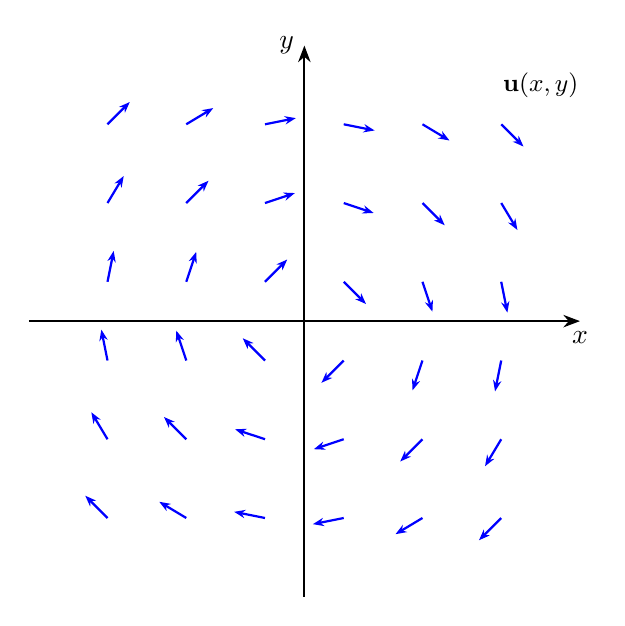
\begin{tikzpicture}
  % Axes
  \draw[axis] (-3.5,0) -- (3.5,0) node[below] {$x$};
  \draw[axis] (0,-3.5) -- (0,3.5) node[left] {$y$};

  % Vector field: (y, -x) showing rotation
  \foreach \x in {-2.5,-1.5,-0.5,0.5,1.5,2.5} {
    \foreach \y in {-2.5,-1.5,-0.5,0.5,1.5,2.5} {
      \pgfmathsetmacro{\norm}{sqrt(\y*\y + \x*\x)}
      \pgfmathsetmacro{\ux}{0.4*\y/max(\norm,0.01)}
      \pgfmathsetmacro{\uy}{0.4*(-\x)/max(\norm,0.01)}
      \draw[-{Stealth[length=4pt]}, blue, thick]
        (\x,\y) -- ++(\ux,\uy);
    }
  }

  % Label
  \node[font=\small] at (3,3) {$\mathbf{u}(x,y)$};
\end{tikzpicture}
\end{document}
